%% LyX 2.3.2 created this file.  For more info, see http://www.lyx.org/.
%% Do not edit unless you really know what you are doing.
\documentclass[english,aspectratio=169,handout]{beamer}
\usepackage{mathptmx}
\usepackage{eulervm}
\usepackage[T1]{fontenc}
\usepackage[latin9]{inputenc}
\usepackage{babel}
\usepackage{amsmath}
\usepackage{amssymb}
\usepackage{graphicx}
\usepackage{dsfont}
\ifx\hypersetup\undefined
  \AtBeginDocument{%
    \hypersetup{unicode=true,pdfusetitle,
 bookmarks=true,bookmarksnumbered=false,bookmarksopen=false,
 breaklinks=false,pdfborder={0 0 0},pdfborderstyle={},backref=false,colorlinks=true,
 allcolors=NYUPurple,urlcolor=LightPurple}
  }
\else
  \hypersetup{unicode=true,pdfusetitle,
 bookmarks=true,bookmarksnumbered=false,bookmarksopen=false,
 breaklinks=false,pdfborder={0 0 0},pdfborderstyle={},backref=false,colorlinks=true,
 allcolors=NYUPurple,urlcolor=LightPurple}
\fi

\makeatletter

%%%%%%%%%%%%%%%%%%%%%%%%%%%%%% LyX specific LaTeX commands.
%% Because html converters don't know tabularnewline
\providecommand{\tabularnewline}{\\}

%%%%%%%%%%%%%%%%%%%%%%%%%%%%%% Textclass specific LaTeX commands.
% this default might be overridden by plain title style
\newcommand\makebeamertitle{\frame{\maketitle}}%
% (ERT) argument for the TOC
\AtBeginDocument{%
  \let\origtableofcontents=\tableofcontents
  \def\tableofcontents{\@ifnextchar[{\origtableofcontents}{\gobbletableofcontents}}
  \def\gobbletableofcontents#1{\origtableofcontents}
}

%%%%%%%%%%%%%%%%%%%%%%%%%%%%%% User specified LaTeX commands.
\usetheme{CambridgeUS} 
\beamertemplatenavigationsymbolsempty


% Set Color ==============================
\definecolor{NYUPurple}{RGB}{87,6,140}
\definecolor{LightPurple}{RGB}{165,11,255}


\setbeamercolor{title}{fg=NYUPurple}
%\setbeamercolor{frametitle}{fg=NYUPurple}
\setbeamercolor{frametitle}{fg=NYUPurple}

\setbeamercolor{background canvas}{fg=NYUPurple, bg=white}
\setbeamercolor{background}{fg=black, bg=NYUPurple}

\setbeamercolor{palette primary}{fg=black, bg=gray!30!white}
\setbeamercolor{palette secondary}{fg=black, bg=gray!20!white}
\setbeamercolor{palette tertiary}{fg=gray!20!white, bg=NYUPurple}

\setbeamertemplate{headline}{}

\setbeamercolor{parttitle}{fg=NYUPurple}
\setbeamercolor{sectiontitle}{fg=NYUPurple}
\setbeamercolor{sectionname}{fg=NYUPurple}
\setbeamercolor{section page}{fg=NYUPurple}

\AtBeginSection[]{
  \begin{frame}
  \vfill
  \centering
\setbeamercolor{section title}{fg=NYUPurple}
 \begin{beamercolorbox}[sep=8pt,center,shadow=true,rounded=true]{title}
    \usebeamerfont{title}\usebeamercolor[fg]{title}\insertsectionhead\par%
  \end{beamercolorbox}
  \vfill
  \end{frame}
}

\makeatother

\begin{document}
\global\long\def\reals{\mathbf{R}}%
 
\global\long\def\integers{\mathbf{Z}}%
 
\global\long\def\naturals{\mathbf{N}}%
 
\global\long\def\rationals{\mathbf{Q}}%
 
\global\long\def\ca{\mathcal{A}}%
 
\global\long\def\cb{\mathcal{B}}%
 
\global\long\def\cc{\mathcal{C}}%
 
\global\long\def\cd{\mathcal{D}}%
 
\global\long\def\ce{\mathcal{E}}%
 
\global\long\def\cf{\mathcal{F}}%
 
\global\long\def\cg{\mathcal{G}}%
 
\global\long\def\ch{\mathcal{H}}%
 
\global\long\def\ci{\mathcal{I}}%
 
\global\long\def\cj{\mathcal{J}}%
 
\global\long\def\ck{\mathcal{K}}%
 
\global\long\def\cl{\mathcal{L}}%
 
\global\long\def\cm{\mathcal{M}}%
 
\global\long\def\cn{\mathcal{N}}%
 
\global\long\def\co{\mathcal{O}}%
 
\global\long\def\cp{\mathcal{P}}%
 
\global\long\def\cq{\mathcal{Q}}%
 
\global\long\def\calr{\mathcal{R}}%
 
\global\long\def\cs{\mathcal{S}}%
 
\global\long\def\ct{\mathcal{T}}%
 
\global\long\def\cu{\mathcal{U}}%
 
\global\long\def\cv{\mathcal{V}}%
 
\global\long\def\cw{\mathcal{W}}%
 
\global\long\def\cx{\mathcal{X}}%
 
\global\long\def\cy{\mathcal{Y}}%
 
\global\long\def\cz{\mathcal{Z}}%
 
\global\long\def\ind#1{1(#1)}%
 %\newcommand{\pr}{P}
\global\long\def\pr{\mathbb{P}}%
 
\global\long\def\predsp{\cy}%
 %{\hat{\cy}}
\global\long\def\outsp{\cy}%

\global\long\def\prxy{P_{\cx\times\cy}}%
 
\global\long\def\prx{P_{\cx}}%
 
\global\long\def\prygivenx{P_{\cy\mid\cx}}%
 %\newcommand{\ex}{E}
\global\long\def\ex{\mathbb{E}}%
 
\global\long\def\var{\textrm{Var}}%
 
\global\long\def\cov{\textrm{Cov}}%
 
\global\long\def\sgn{\textrm{sgn}}%
 
\global\long\def\sign{\textrm{sign}}%
 
\global\long\def\kl{\textrm{KL}}%
 
\global\long\def\law{\mathcal{L}}%
 
\global\long\def\eps{\varepsilon}%
 
\global\long\def\as{\textrm{ a.s.}}%
 
\global\long\def\io{\textrm{ i.o.}}%
 
\global\long\def\ev{\textrm{ ev.}}%
 
\global\long\def\convd{\stackrel{d}{\to}}%
 
\global\long\def\eqd{\stackrel{d}{=}}%
 
\global\long\def\del{\nabla}%
 
\global\long\def\loss{\ell}%
 
\global\long\def\risk{R}%
 
\global\long\def\emprisk{\hat{R}}%
 
\global\long\def\lossfnl{L}%
 
\global\long\def\emplossfnl{\hat{L}}%
 
\global\long\def\empminimizer#1{\hat{#1}^{*}}%
 
\global\long\def\minimizer#1{#1^{*}}%
\global\long\def\optimizer#1{#1^{*}}%
 
\global\long\def\etal{\textrm{et. al.}}%
 
\global\long\def\tr{\operatorname{tr}}%

\global\long\def\trace{\operatorname{trace}}%
 
\global\long\def\diag{\text{diag}}%
 
\global\long\def\rank{\text{rank}}%
 
\global\long\def\linspan{\text{span}}%
 
\global\long\def\spn{\text{span}}%
 
\global\long\def\proj{\text{Proj}}%
 
\global\long\def\argmax{\operatornamewithlimits{arg\, max}}%
 
\global\long\def\argmin{\operatornamewithlimits{arg\, min}}%

\global\long\def\bfx{\mathbf{x}}%
 
\global\long\def\bfy{\mathbf{y}}%
 
\global\long\def\bfl{\mathbf{\lambda}}%
 
\global\long\def\bfm{\mathbf{\mu}}%
 
\global\long\def\calL{\mathcal{L}}%

\global\long\def\vw{\boldsymbol{w}}%
 
\global\long\def\vx{\boldsymbol{x}}%
 
\global\long\def\vxi{\boldsymbol{\xi}}%
 
\global\long\def\valpha{\boldsymbol{\alpha}}%
 
\global\long\def\vbeta{\boldsymbol{\beta}}%
 
\global\long\def\vsigma{\boldsymbol{\sigma}}%
\global\long\def\vtheta{\boldsymbol{\theta}}%
 
\global\long\def\vd{\boldsymbol{d}}%
 
\global\long\def\vs{\boldsymbol{s}}%
 
\global\long\def\vt{\boldsymbol{t}}%
 
\global\long\def\vh{\boldsymbol{h}}%
 
\global\long\def\ve{\boldsymbol{e}}%
 
\global\long\def\vf{\boldsymbol{f}}%
 
\global\long\def\vg{\boldsymbol{g}}%
 
\global\long\def\vz{\boldsymbol{z}}%
 
\global\long\def\vk{\boldsymbol{k}}%
 
\global\long\def\va{\boldsymbol{a}}%
 
\global\long\def\vb{\boldsymbol{b}}%
 
\global\long\def\vv{\boldsymbol{v}}%
 
\global\long\def\vy{\boldsymbol{y}}%

\global\long\def\dom{\textrm{\textbf{dom} }}%
\global\long\def\rank{\text{\textbf{rank }}}%
\global\long\def\conv{\textrm{\textbf{conv} }}%
\global\long\def\relint{\text{\textbf{relint }}}%
\global\long\def\aff{\text{\textbf{aff }}}%

\global\long\def\hil{\ch}%
 
\global\long\def\rkhs{\hil}%
 
\global\long\def\ber{\text{Ber}}%

\title[DS-GA 1003 / CSCI-GA 2567]{Review: MLE and Conditional Probability Models}
\author{Xintian Han \& David S. Rosenberg }
\date{March 5, 2019}
\institute{CDS, NYU}

\makebeamertitle
\mode<article>{Just in article version}

\begin{frame}{Contents}

\tableofcontents{}
\end{frame}
\section{Maximum Likelihood}
\begin{frame}{Maximum Likelihood Estimation}
\begin{itemize}
\item Suppose $\cd=\left(y_{1},\ldots,y_{n}\right)$ is an i.i.d. sample
from some distribution. 
\end{itemize}
\begin{definition}
A \textbf{maximum likelihood estimator (MLE)} for $\theta$ in the
model $\left\{ p(y;\theta)\mid\theta\in\Theta\right\} $ is
\begin{eqnarray*}
\hat{\theta} & \in & \argmax_{\theta\in\Theta}\log p(\cd,\hat{\theta})\\
 & = & \argmax_{\theta\in\Theta}\sum_{i=1}^{n}\log p(y_{i};\theta).
\end{eqnarray*}
\end{definition}

\end{frame}
%
\begin{frame}{Maximum Likelihood Estimation}
\begin{itemize}
\item Finding the MLE is an \textbf{optimization problem}.
\end{itemize}

\begin{itemize}
\item For some model families, calculus gives a closed form for the MLE.
\end{itemize}

\begin{itemize}
\item Can also use numerical methods we know (e.g. SGD). 
\end{itemize}
\end{frame}
%
\begin{frame}{MLE Existence}
\begin{itemize}
\item In certain situations, the MLE may not exist. 
\item But there is usually a good reason for this.
\end{itemize}

\begin{itemize}
\item e.g. Gaussian family $\left\{ \cn(\mu,\sigma^{2})\mid\mu\in\reals,\sigma^{2}>0\right\} $
\item We have a single observation $y$. 
\item Is there an MLE?
\end{itemize}

\begin{itemize}
\item Taking $\mu=y$ and $\sigma^{2}\to0$ drives likelihood to infinity. 
\item MLE doesn't exist.
\end{itemize}
\end{frame}
%
\begin{frame}{Example: MLE for Poisson}
\begin{itemize}
\item Observed counts $\cd=\left(k_{1},\ldots,k_{n}\right)$ for taxi cab
pickups over $n$ weeks.
\begin{itemize}
\item $k_{i}$ is number of pickups at Penn Station Mon, 7-8pm, for week
$i$.
\end{itemize}
\item We want to fit a Poisson distribution to this data.

\item The Poisson log-likelihood for a single count is
\begin{eqnarray*}
\log\left[p(k;\lambda)\right] & = & \log\left[\frac{\lambda^{k}e^{-\lambda}}{k!}\right]\\
 & = & k\log\lambda-\lambda-\log\left(k!\right)
\end{eqnarray*}


\item The full log-likelihood is
\begin{eqnarray*}
\log p(\cd,\lambda) & = & \sum_{i=1}^{n}\left[k_{i}\log\lambda-\lambda-\log\left(k_{i}!\right)\right].
\end{eqnarray*}
 
\end{itemize}
\end{frame}

\begin{frame}{Example: MLE for Poisson}

\begin{itemize}
\item The full log-likelihood is
\begin{eqnarray*}
\log p(\cd,\lambda) & = & \sum_{i=1}^{n}\left[k_{i}\log\lambda-\lambda-\log\left(k_{i}!\right)\right]
\end{eqnarray*}


\item First order condition gives
\begin{eqnarray*}
0=\frac{\partial}{\partial\lambda}\left[\log p(\cd,\lambda)\right] & = & \sum_{i=1}^{n}\left[\frac{k_{i}}{\lambda}-1\right]\\
\implies\lambda & = & \frac{1}{n}\sum_{i=1}^{n}k_{i}
\end{eqnarray*}


\item So MLE $\hat{\lambda}$ is just the mean of the counts. 
\end{itemize}
\end{frame}

\begin{frame}{Estimating Distributions, Overfitting, and Hypothesis Spaces}

\begin{itemize}
\item Just as in classification and regression, MLE can overfit! 

\item Example Probability Models:
\begin{itemize}
\item $\cf=\left\{ \text{Poisson distributions}\right\} $.
\item $\cf=\left\{ \text{Negative binomial distributions}\right\} $.

\item $\cf=$$\left\{ \text{Histogram with 10 bins}\right\} $
\item $\cf=$$\left\{ \text{Histogram with bin for every \ensuremath{y\in\cy}}\right\} $
{[}will likely overfit for continuous data{]} 

\end{itemize}
\item How to judge which model works the best?

\item Choose the model with the \textbf{highest likelihood on validation
set}.
\end{itemize}
\end{frame}
\section{Bernoulli Regression}
\begin{frame}{Probabilistic Binary Classifiers}
\begin{itemize}
\item Setting: $\cx=\reals^{d}$, $\cy=\left\{ 0,1\right\} $

\item For each $x$, need to predict a distribution on $\cy=\left\{ 0,1\right\} $.
\item How can we define a distribution supported on $\left\{ 0,1\right\} $?

\item Sufficient to specify the \textbf{Bernoulli parameter} $\theta=p(y=1)$.

\item We can refer to this distribution as $\text{Bernoulli}(\theta)$.
\end{itemize}
\end{frame}
%
\begin{frame}{Linear Probabilistic Classifiers}
\begin{itemize}
\item Setting: $\cx=\reals^{d}$, $\cy=\left\{ 0,1\right\} $
\item Want prediction function to map each $x\in\reals^{d}$ to $\theta\in\left[0,1\right]$.

\item We first \textbf{extract} \textbf{information }from $x\in\reals^{d}$
and summarize in a single number.
\begin{itemize}
\item That number is analogous to the \textbf{score} in classification.

\end{itemize}
\item For a \textbf{linear method}, this extraction is done with a linear
function:
\[
\underbrace{x}_{\in\reals^{d}}\mapsto\underbrace{w^{T}x}_{\in\reals}
\]


\item As usual, $x\mapsto w^{T}x$ will include affine functions if we include
a constant feature in $x$.

\item $w^{T}x$ is called the \textbf{linear predictor. }
\item Still need to map this to $[0,1]$.
\end{itemize}
\end{frame}
%
\begin{frame}{The Transfer Function}
\begin{itemize}
\item Need a function to map the linear predictor in $\reals$ to $\left[0,1\right]$:
\[
\underbrace{x}_{\in\reals^{d}}\mapsto\underbrace{w^{T}x}_{\in\reals}\mapsto\underbrace{f(w^{T}x)}_{\in[0,1]}=\theta,
\]
where $f:\reals\to[0,1]$. We'll call $f$ the \textbf{transfer }function.
\end{itemize}

\begin{itemize}
\item So prediction function is $x\mapsto f(w^{T}x)$. 
\end{itemize}

\end{frame}
%
\begin{frame}{Transfer Functions for Bernoulli}

\begin{itemize}
\item Two commonly used transfer functions to map from $w^{T}x$ to $\theta$:
\end{itemize}
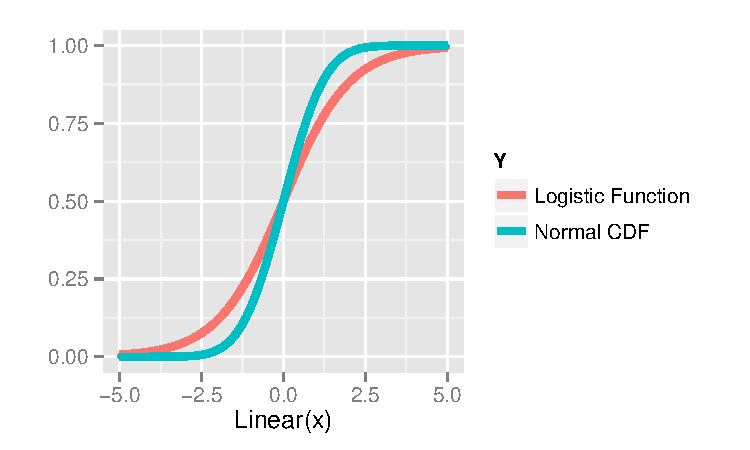
\includegraphics[width=0.6\textwidth]{../Figures/GLM/bernoulliInverseLinkFunctions}
\begin{itemize}
\item Logistic function: $f(\eta)=\frac{1}{1+e^{-\eta}}$ $\implies$
Logistic Regression
\item Normal CDF $f(\eta)=\int_{-\infty}^{\eta}\frac{1}{\sqrt{2\pi}}e^{-x^{2}/2}$$\implies$
Probit Regression
\end{itemize}
\end{frame}
%
\begin{frame}{Learning}

\begin{itemize}
\item Input space $\cx=\reals^{d}$
\item Outcome space $\cy=\left\{ 0,1\right\} $

\item Action space $\ca=[0,1]$ (Representing Bernoulli$(\theta)$ distributions
by $\theta\in\left[0,1\right]$)

\item Hypothesis space $\cf=\left\{ x\mapsto f(w^{T}x)\mid w\in\reals^{d}\right\} $ 

\item Parameter space $\reals^{d}$ (Each prediction function represented
by $w\in\reals^{d}.)$

\item We can choose $w$ using maximum likelihood...
\end{itemize}
\end{frame}

%
\begin{frame}{A Clever Way To Write $\hat{p}(y\mid x;w)$}
\begin{itemize}
\item For a given $x,w\in\reals^{d}$ and $y\in\left\{ 0,1\right\} $, the
likelihood of $w$ for $\left(x,y\right)$ is
\[
p(y\mid x;w)=\begin{cases}
f(w^{T}x) & y=1\\
1-f(w^{T}x) & y=0
\end{cases}
\]
\end{itemize}

\begin{itemize}
\item It will be convenient to write this as
\[
p(y\mid x;w)=\left[f(w^{T}x)\right]^{y}\left[1-f(w^{T}x)\right]^{1-y},
\]
which is obvious as long as you remember $y\in\left\{ 0,1\right\} $.
\end{itemize}
\end{frame}
%
\begin{frame}{Bernoulli Regression: Likelihood Scoring}
\begin{itemize}
\item Suppose we have data $\cd:\;(x_{1},y_{1}),\ldots,(x_{n},y_{n})\in\reals^{d}\times\left\{ 0,1\right\} $.

\item The likelihood of $w\in\reals^{d}$ for data $\cd$ is
\begin{eqnarray*}
p(\cd;w) & = & \prod_{i=1}^{n}p(y_{i}\mid x_{i};w)\text{ [by independence]}\\
 & = & \prod_{i=1}^{n}\left[f(w^{T}x_{i})\right]^{y_{i}}\left[1-f(w^{T}x_{i})\right]^{1-y_{i}}.
\end{eqnarray*}


\item Easier to work with the log-likelihood:
\[
\log p(\cd;w)=\sum_{i=1}^{n}\left(y_{i}\log f(w^{T}x_{i})+\left(1-y_{i}\right)\log\left[1-f(w^{T}x_{i})\right]\right)
\]
\end{itemize}
\end{frame}
%
\begin{frame}{Bernoulli Regression: MLE}
\begin{itemize}
\item Maximum Likelihood Estimation (MLE) finds $w$ maximizing $\log p(\cd,w)$.

\item Equivalently, minimize the \textbf{negative log-likelihood} objective
function
\[
J(w)=-\left[\sum_{i=1}^{n}y_{i}\log f(w^{T}x_{i})+\left(1-y_{i}\right)\log\left[1-f(w^{T}x_{i})\right]\right].
\]


\item For differentiable $f$,
\begin{itemize}
\item $J(w)$ is differentiable, and we can use SGD.
\item What guarantees us to find the global minima of $J(w)$ by SGD?
\pause{}
\item Convexity of $J(w)$!
\end{itemize}
\end{itemize}
\end{frame}

\section{Poisson Regression}

\global\long\def\poi{\text{Poisson}}%

\begin{frame}{Poisson Regression: Setup}
\begin{itemize}
\item Input space $\cx=\reals^{d}$, Output space $\cy=\left\{ 0,1,2,3,4,\dots\right\} $

\item In Poisson regression, prediction functions produce a Poisson distribution.
\begin{itemize}
\item Represent Poisson$\left(\lambda\right)$ distribution by the mean
parameter $\lambda\in\left(0,\infty\right)$.

\end{itemize}
\item Action space $\ca=\left(0,\infty\right)$

\item In Poisson regression, $x$ enters \textbf{linearly:} $x\mapsto\underbrace{w^{T}x}_{\reals}\mapsto\lambda=\underbrace{f(w^{T}x)}_{(0,\infty)}$.

\item What can we use as the transfer function $f:\reals\to\left(0,\infty\right)$?
\end{itemize}
\end{frame}
%
\begin{frame}{Poisson Regression: Transfer Function}
\begin{itemize}
\item In Poisson regression, $x$ enters \textbf{linearly:} 
\[
x\mapsto\underbrace{w^{T}x}_{\reals}\mapsto\lambda=\underbrace{f(w^{T}x)}_{(0,\infty)}.
\]
\item Standard approach is to take
\[
f(w^{T}x)=\exp\left(w^{T}x\right).
\]


\item Note that range of $f(w^{T}x)\in\left(0,\infty\right)$, (appropriate
for the Poisson parameter).
\end{itemize}
\end{frame}
%
\begin{frame}{Poisson Regression: Likelihood Scoring}
\begin{itemize}
\item Suppose we have data $\cd=\left\{ (x_{1},y_{1}),\ldots,(x_{n},y_{n})\right\} $.
\item Recall the log-likelihood for Poisson parameter $\lambda_{i}$ on
observation $y_{i}$ is:
\begin{eqnarray*}
\log p(y_{i};\lambda_{i}) & = & \left[y_{i}\log\lambda_{i}-\lambda_{i}-\log\left(y_{i}!\right)\right]
\end{eqnarray*}


\item Now we want to predict a different $\lambda_{i}$ for every $x_{i}$
with the model
\[
\lambda_{i}=f(w^{T}x_{i})=\exp\left(w^{T}x_{i}\right).
\]


\item The likelihood for $w$ on the full dataset $\cd$ is
\begin{eqnarray*}
\log p(\cd;w) & = & \sum_{i=1}^{n}\left[y_{i}\log\left[\exp\left(w^{T}x_{i}\right)\right]-\exp\left(w^{T}x_{i}\right)-\log\left(y_{i}!\right)\right]\\
 & = & \sum_{i=1}^{n}\left[y_{i}w^{T}x_{i}-\exp\left(w^{T}x_{i}\right)-\log\left(y_{i}!\right)\right]
\end{eqnarray*}
\end{itemize}
\end{frame}
%
\begin{frame}{Poisson Regression: MLE}
\begin{itemize}
\item To get MLE, need to maximize 
\[
J(w)=\log p(\cd;w)=\sum_{i=1}^{n}\left[y_{i}w^{T}x_{i}-\exp\left(w^{T}x_{i}\right)-\log\left(y_{i}!\right)\right]
\]
 over $w\in\reals^{d}$.
\end{itemize}

\begin{itemize}
\item No closed form for optimum, but it's concave, so easy to optimize. 
\end{itemize}
\end{frame}
%
\begin{frame}{Poisson Regression Example}

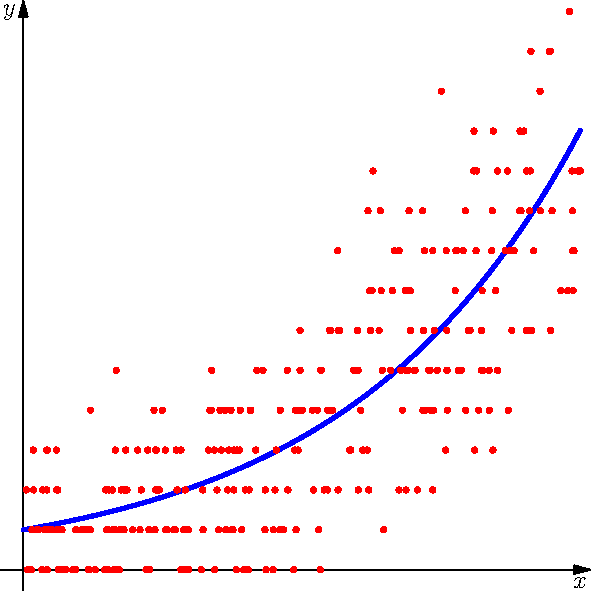
\includegraphics[height=0.55\paperheight]{../Figures/conditional-probability-models/poissonBumps2}
\begin{itemize}
\item Example application: Phone call counts per day for a startup company,
over 300 days.

\item Blue line is mean $\mu(x)=\exp\left(wx\right)$, some $w\in\reals$.
(Only linear part $x\mapsto wx$ is learned.)

\item Samples are $y_{i}\sim\text{Poisson}(wx_{i})$. \let\thefootnote\relax\footnotetext{\tiny{Plot courtesy of Brett Bernstein.}}
\end{itemize}
\end{frame}
%
\begin{frame}{Nonlinear Score Function: Sneak Preview}
 

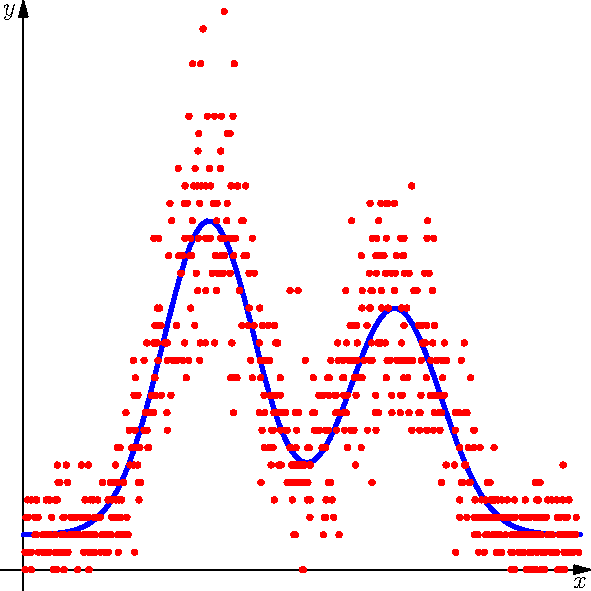
\includegraphics[height=0.55\paperheight]{../Figures/conditional-probability-models/poissonBumps}
\begin{itemize}
\item Blue line is mean $\mu(x)=\exp\left(f(x)\right)$, for some nonlinear
$f$ learned from data.

\item Samples are $y_{i}\sim\text{Poisson}(\exp\left(f(x_{i})\right)$.

\item We can do this with gradient boosting and neural networks, coming
up in a few weeks. \let\thefootnote\relax\footnotetext{\tiny{Plot courtesy of Brett Bernstein.}}
\end{itemize}
\end{frame}
%

\section{Conditional Gaussian Regression}
\begin{frame}{Gaussian Linear Regression}
\begin{itemize}
\item Input space $\cx=\reals^{d}$, Output space $\cy=\reals$

\item In Gaussian regression, prediction functions produce a distribution
$\cn(\mu,\sigma^{2})$.
\begin{itemize}
\item Assume $\sigma^{2}$ is known.
\end{itemize}
\item Represent $\cn(\mu,\sigma^{2})$ by the mean parameter $\mu\in\reals$.

\item Action space $\ca=\reals$

\item In Gaussian linear regression, $x$ enters \textbf{linearly:} $x\mapsto\underbrace{w^{T}x}_{\reals}\mapsto\mu=\underbrace{f(w^{T}x)}_{\reals}$.

\item Since $\mu\in\reals$, we can take the identity transfer function:
$f(w^{T}x)=w^{T}x$.
\end{itemize}
\end{frame}
%
\begin{frame}{Gaussian Regression: Likelihood Scoring}
\begin{itemize}
\item Suppose we have data $\cd=\left\{ (x_{1},y_{1}),\ldots,(x_{n},y_{n})\right\} $.
\item Compute the model likelihood for $\cd$:
\begin{align*}
p(\cd;w)= & \prod_{i=1}^{n}p(y_{i}\mid x_{i};w)\text{ [by independence]}
\end{align*}


\item Maximum Likelihood Estimation (MLE) finds $w$ maximizing $\hat{p}(\cd;w)$.
\item Equivalently, maximize the data log-likelihood:
\[
\minimizer w=\argmax_{w\in\reals^{d}}\sum_{i=1}^{n}\log p(y_{i}\mid x_{i};w)
\]

\item Let's start solving this!
\end{itemize}
\end{frame}
%
\begin{frame}{Gaussian Regression: MLE}
\begin{itemize}
\item The conditional log-likelihood is:
\begin{eqnarray*}
 &  & \sum_{i=1}^{n}\log p(y_{i}\mid x_{i};w)\\
 & = & \sum_{i=1}^{n}\log\left[\frac{1}{\sigma\sqrt{2\pi}}\exp\left(-\frac{(y_{i}-w^{T}x_{i})^{2}}{2\sigma^{2}}\right)\right]\\
 & = & \underbrace{\sum_{i=1}^{n}\log\left[\frac{1}{\sigma\sqrt{2\pi}}\right]}_{\mbox{independent of }w}+\sum_{i=1}^{n}\left(-\frac{(y_{i}-w^{T}x_{i})^{2}}{2\sigma^{2}}\right)
\end{eqnarray*}


\begin{itemize}
\item MLE is the $w$ where this is maximized.

\item Note that $\sigma^{2}$ is irrelevant to finding the maximizing $w$.

\item Can drop the negative sign and make it a minimization problem.
\end{itemize}
\end{itemize}
\end{frame}
%
\begin{frame}{Gaussian Regression: MLE}
\begin{itemize}
\item The MLE is 
\begin{align*}
\minimizer w= & \argmin_{w\in\reals^{d}}\sum_{i=1}^{n}(y_{i}-w^{T}x_{i})^{2}
\end{align*}


\item This is exactly the objective function for least squares. 

\item From here, can use usual approaches to solve for $w^{*}$ (SGD, linear
algebra, calculus, etc.) 
\end{itemize}

\end{frame}
%

\section{Multinomial Logistic Regression}
\begin{frame}{Multinomial Logistic Regression}
\begin{itemize}
\item Setting: $\cx=\reals^{d}$, $\cy=\left\{ 1,\ldots,k\right\} $
\end{itemize}

\begin{itemize}
\item For each $x$, we want to produce a distribution on $k$ classes.
\end{itemize}

\begin{itemize}
\item Such a distribution is called a ``\textbf{multinoulli}'' or ``\textbf{categorical}''
distribution.
\end{itemize}

\begin{itemize}
\item Represent categorical distribution by probability vector $\theta=\left(\theta_{1},\ldots,\theta_{k}\right)\in\reals^{k}$:
\begin{itemize}
\item $\sum_{i=1}^{k}\theta_{i}=1$ and $\theta_{i}\ge0$ for $i=1,\ldots,k$
(i.e. $\theta$ represents a \textbf{distribution}) and
\end{itemize}

\item So $\forall y\in\left\{ 1,\ldots,k\right\} $, $p(y)=\theta_{y}$.
\end{itemize}
\end{frame}
%
\begin{frame}{Multinomial Logistic Regression}
\begin{itemize}
\item From each $x$, we compute a linear score function for each class:
\[
x\mapsto\left(\left\langle w_{1},x\right\rangle ,\ldots,\left\langle w_{k},x\right\rangle \right)\in\reals^{k},
\]
where we've introduced parameter vectors $w_{1},\ldots,w_{k}\in\reals^{d}$.

\item We need to map this $\reals^{k}$ vector of scores into a probability
vector.

\item Consider the \textbf{softmax function:
\[
\left(s_{1},\ldots,s_{k}\right)\mapsto\theta=\left(\frac{e^{s_{1}}}{\sum_{i=1}^{k}e^{s_{i}}},\ldots,\frac{e^{s_{k}}}{\sum_{i=1}^{k}e^{s_{i}}}\right).
\]
}

\item Note that $\theta\in\reals^{k}$ and
\begin{eqnarray*}
\theta_{i} & > & 0\qquad i=1,\ldots,k\\
\sum_{i=1}^{k}\theta_{i} & = & 1
\end{eqnarray*}
\end{itemize}
\end{frame}
%
\begin{frame}{Multinomial Logistic Regression}
\begin{itemize}
\item Say we want to get the predicted categorical distribution for a given
$x\in\reals^{d}$. 
\item First compute the scores $(\in\reals^{k})$ and then their softmax:
\textbf{
\[
x\mapsto\left(\left\langle w_{1},x\right\rangle ,\ldots,\left\langle w_{k},x\right\rangle \right)\mapsto\theta=\left(\frac{\exp\left(w_{1}^{T}x\right)}{\sum_{i=1}^{k}\exp\left(w_{i}^{T}x\right)},\ldots,\frac{\exp\left(w_{k}^{T}x\right)}{\sum_{i=1}^{k}\exp\left(w_{i}^{T}x\right)}\right)
\]
}
\end{itemize}

\begin{itemize}
\item We can write the conditional probability for any $y\in\left\{ 1,\ldots,k\right\} $
as
\[
p(y\mid x;w)=\frac{\exp\left(w_{y}^{T}x\right)}{\sum_{i=1}^{k}\exp\left(w_{i}^{T}x\right)}.
\]
\end{itemize}
\end{frame}
%
\begin{frame}{Multinomial Logistic Regression}
\begin{itemize}
\item Putting this together, we write multinomial logistic regression as
\[
p(y\mid x;w)=\frac{\exp\left(w_{y}^{T}x\right)}{\sum_{i=1}^{k}\exp\left(w_{i}^{T}x\right)}.
\]


\item How do we do learning here? What parameters are we estimating?

\item Our model is specified once we have $w_{1},\ldots,w_{k}\in\reals^{d}$.
\item Find parameter settings maximizing the log-likelihood of data $\cd$.

\item This objective function is concave in $w$'s and straightforward to
optimize.
\end{itemize}
\end{frame}

\section{Maximum Likelihood as ERM}
\begin{frame}{Conditional Probability Modeling as Statistical Learning}

\begin{itemize}
\item Input space $\cx$
\item Outcome space $\cy$
\item All pairs $(x,y)$ are independent with distribution $P_{\cx\times\cy}$. 

\item \textbf{Action space} $\ca=\left\{ p(y)\mid p\text{ is a probability density or mass function on }\cy\right\} $.

\item Hypothesis space $\cf$ contains decision functions $f:\cx\to\ca$. 

\item Maximum likelihood estimation for dataset $\cd=\left((x_{1},y_{1}),\ldots,(x_{n},y_{n}\right)$
is
\[
\hat{f}_{\text{MLE}}\in\argmax_{f\in\cf}\sum_{i=1}^{n}\log\left[f(x_{i})(y_{i})\right]
\]

\end{itemize}
\end{frame}
%
\begin{frame}{Conditional Probability Modeling as Statistical Learning}

\begin{itemize}
\item Take loss $\ell:\ca\times\cy\to\reals$ for a predicted PDF or PMF
$p(y)$ and outcome $y$ to be
\[
\ell(p,y)=-\log p(y)
\]


\item The risk of decision function $f:\cx\to\ca$ is
\[
R(f)=-\ex_{x,y}\log\left[f(x)(y)\right],
\]
where $f(x)$ is a PDF or PMF on $\cy$, and we're evaluating it on
$y$.
\end{itemize}
\end{frame}
%
\begin{frame}{Conditional Probability Modeling as Statistical Learning}
\begin{itemize}
\item The empirical risk of $f$ for a sample $\cd=\left\{ y_{1},\ldots,y_{n}\right\} \in\cy$
is 
\[
\hat{R}(f)=-\frac{1}{n}\sum_{i=1}^{n}\log\left[f(x_{i})\right](y_{i}).
\]
This is called the negative \textbf{conditional log-likelihood}.
\end{itemize}

\begin{itemize}
\item Thus for the negative log-likelihood loss, ERM and MLE are equivalent
\end{itemize}
\end{frame}

\section{Review Questions}
\begin{frame}{Maximum Likelihood}
\begin{enumerate}
\item Suppose we have samples $x_1, \dots, x_n$ i.i.d drawn from Bernoulli($p$). Find the maximum likelihood estimator of $p$.
\item  Suppose we have samples $x_1, \dots, x_n$ i.i.d drawn from uniform distribution $\mathcal{U}(a,b)$. Find the maximum likelihood estimator of $a$ and $b$.	
\end{enumerate}	
\end{frame}

\begin{frame}{Maximum Likelihood}
\begin{itemize}
\item Suppose we have samples $x_1, \dots, x_n$ i.i.d drawn from Bernoulli($p$). Find the maximum likelihood estimator of $p$.
\item[] \textbf{Solution:}
\begin{itemize}
\item The likelihood is:
\[
L(p) = \Pi_{i=1}^n p^{x_i} (1-p)^{(1-x_i)}.
\]	
\pause{}
\item The log-likelihood is:
\[
\ell(p) = \log p \sum_{i=1}^n x_i + \log (1-p) \sum_{i=1}^n(1-x_i).
\]
\pause{}
\item Set the derivative of log-likelihood w.r.t. $p$ to zero:
\[
\frac{\partial \ell(p)}{\partial p} = \frac{\sum_{i=1}^n x_i}{p} - \frac{\sum_{i=1}^n(1-x_i)}{1-p} = 0.
\]
\end{itemize}
\end{itemize}

	
\end{frame}

\begin{frame}{Maximum Likelihood}
\begin{itemize}
\item Solving the equation above, we have:
\[
p = \frac{1}{n} \sum_{i=1}^n x_i.
\]
\pause{}
\item The second derivative of log-likelihood w.r.t. $p$ is 
\[
\frac{\partial^2\ell(p)}{\partial p^2} = \frac{-\sum_{i=1}^n x_i}{p^2} -\frac{ \sum_{i=1}^n(1-x_i)}{(1-p)^2}.
\]
\item Since $p \in [0,1]$ and $x_i \in \{0,1\}$, the second derivative is always negative. The log-likelihood is concave. Therefore, $p =\frac{1}{n} \sum_{i=1}^n x_i $ gives us the MLE.		
\item A twice differentiable function of one variable is concave on an interval if and only if its second derivative is non-positive there!
\item Why cannot we have the same closed form solution for logistic regression?
\end{itemize}
\end{frame}

\begin{frame}{Maximum Likelihood}
\begin{itemize}
\item Suppose we have samples $x_1, \dots, x_n$ i.i.d drawn from uniform distribution $\mathcal{U}(a,b)$. Find the maximum likelihood estimator of $a$ and $b$.	
\item[] \textbf{Solution:}
\pause{}
\begin{itemize}
\item The likelihood is:
\[
L(a,b) = \Pi_{i=1}^n \left(\frac{1}{b-a} \mathds{1}_{[a,b]}(x_i)\right)
\]	
\item Let $x_{(1)},\dots, x_{(n)}$ be the order statistics. 
\item The likelihood is greater than zero if and only $a < x_{(1)}$ and $b>x_{(n)}$. 
\item When $a<x_{(1)}$ and $b>x_{(n)}$, the likelihood is a monotonically decreasing function of $(b-a)$. 
\item And the smallest $(b-a)$ will be attained when $b = x_{(n)}$ and $a = x_{(1)}$. 
\item Therefore, $b = x_{(n)}$ and $a = x_{(1)}$ give us the MLE.
\end{itemize}
\end{itemize}
\end{frame}

\begin{frame}{Maximum Likelihood}
\begin{enumerate}
\item We want to fit a regression model where
  $Y|X=x\sim\mathcal{U}([0,e^{w^Tx}])$ for some $w\in\reals^d$.  Given
  i.i.d.~data points $(X_1,Y_1),\dots,(X_n,Y_n)\in\reals^d\times\reals$,
  give a convex optimization problem that finds the MLE for $w$.	
  \item Suppose we have input-output pairs $\{(x_1,y_1), \dots, (x_n,y_n)\}$, where $x_i \in \mathbb{R}^p$ and $y_i \in N = \{0,1,2,3,\dots\}$ for $i=1,..,n$. Our task is to train a Poisson regression to model the data. Assume the linear coefficients in the model is $w$.
\begin{enumerate}
\item  Suppose a test point $x^*$ is orthogonal to the space generated by the training data. What is the prediction $\ell_2$ regularized Poisson GLM make on the test point?
\item Will the solution of the parameters $\hat{w}$ still be sparse when we use $\ell_1$ regularization?
\end{enumerate}
\end{enumerate}
\end{frame}

\begin{frame}{Maximum Likelihood}
\begin{itemize}
\item We want to fit a regression model where
  $Y|X=x\sim\mathcal{U}([0,e^{w^Tx}])$ for some $w\in\reals^d$.  Given
  i.i.d.~data points $(X_1,Y_1),\dots,(X_n,Y_n)\in\reals^d\times\reals$,
  give a convex optimization problem that finds the MLE for $w$.	
\item [] \textbf{Solution:}
\pause{}
The likelihood $L$ is given by
  $$L(w;x_1,y_1,\dots,x_n,y_n) = \Pi_{i=1}^n \frac{\mathds{1}(y_i\leq
  e^{w^Tx_i})}{e^{w^Tx_i}}.$$
  \pause{}
Taking logs we get
  $$-\sum_{i=1}^n w^Tx_i = -w^T\left(\sum_{i=1}^n x_i\right)$$
  if $y_i\leq \exp(w^Tx_i)$ for all $i$, or $-\infty$ otherwise.  
  \pause{}
  Thus we obtain the linear program
\begin{align*}
    \text{minimize} \quad& w^T\left(\sum_{i=1}^n x_i\right)\\
    \text{subject to} \quad& \log(y_i)\leq w^Tx_i\quad\text{for $i=1,\dots,n$.}
  \end{align*}
\end{itemize}
\end{frame}

\begin{frame}{Maximum Likelihood}
\begin{itemize}
\item Suppose we have input-output pairs $\{(x_1,y_1), \dots, (x_n,y_n)\}$, where $x_i \in \mathbb{R}^p$ and $y_i \in N = \{0,1,2,3,\dots\}$ for $i=1,..,n$. Our task is to train a Poisson regression to model the data. Assume the linear coefficients in the model is $w$.
\begin{itemize}
\item  Suppose a test point $x^*$ is orthogonal to the space generated by the training data. What is the prediction $\ell_2$ regularized Poisson GLM make on the test point?	
\item[] \textbf{Solution:} 
$\ell_2$ penalized Poisson regression objective:
\[
\hat{J}(w)=-\sum_{i=1}^{n}\left[y_{i}w^{T}x_{i}-\exp\left(w^{T}x_{i}\right)-\log\left(y_{i}!\right)\right] + \lambda \|w\|_2^2
\]
\pause{}
From Representer Theorem, the minimizer $\hat{w} = \sum_{i=1}^n \alpha_i x_i$. The prediction is \[
\exp(w^T x^*) = \exp( \sum_{i=1}^n \alpha_i x_i^Tx^*) =\exp(0) = 1
\]
\end{itemize}
\end{itemize}	
\end{frame}

\begin{frame}{Maximum Likelihood}
\begin{itemize}
\item Suppose we have input-output pairs $\{(x_1,y_1), \dots, (x_n,y_n)\}$, where $x_i \in \reals{R}^p$ and $y_i \in N = \{0,1,2,3,\dots\}$ for $i=1,..,n$. Our task is to train a Poisson regression to model the data. Assume the linear coefficients in the model is $w$.
\begin{itemize}
\item  Will the solution of the parameters $\hat{w}$ still be sparse when we use $\ell_1$ regularization?
\pause{}
\item[] \textbf{Solution:} 
Negative log-likelihood of Poisson regression is a convex function. The sublevel set is a convex set. The level set is the boundary of the sublevel set. When the level set approaches the diamond (level set of the $\ell_1$ norm), it is still likely to hit the corner of the diamond.
\end{itemize}
\end{itemize}	
\end{frame}
\end{document}
